\documentclass[11pt,a4paper]{article}
\usepackage[T1]{fontenc}
\usepackage[margin=2.3cm]{geometry}
\usepackage{amsmath,amssymb}
\usepackage{graphicx}
\usepackage[dvipsnames]{xcolor}
\usepackage{enumitem}
\usepackage[colorlinks=true,linkcolor=blue,urlcolor=blue]{hyperref}
\setlength{\parskip}{0.6em}
\setlength{\parindent}{0pt}
\begin{document}

\begin{center}{\LARGE\bfseries openclassifier}\\[0.4em]{\large Draw decision boundaries and read a confusion matrix, in five sessions.}\\[0.2em]\small PAN IIT OSS explainer \textbullet{} higher secondary to advanced undergraduate (levels 4-6)\end{center}

\section*{Why this exists}
Every automatic decision, from a spam filter to a screening test, is a classifier: a rule that splits cases into groups. This explainer shows how such rules are drawn and, more importantly, how to judge them honestly, using only counting, a few formulas and Python.

\section*{The end goal}
Draw decision boundaries and read a confusion matrix. The end goal is to draw decision boundaries and read a confusion matrix: to see what a classifier decides, to count how it fails, and to ask the right questions (what is the base rate, what do the mistakes cost, was this tested on new data) before trusting a number. All examples use synthetic data and are for education only.

\section*{How the five sessions build up}
\begin{enumerate}[nosep]
\item \textbf{Session 1: A rule that splits two groups} (Level 1, conceptual interactive model, 60 min).
\item \textbf{Session 2: Trees, neighbours and the confusion matrix} (Level 2, mathematical engineering model, 90 min).
\item \textbf{Session 3: Judging a classifier honestly} (Level 3, simulation and validation, 90 min).
\item \textbf{Session 4: Tune the forest by cross-validation} (Level 3, simulation and validation, 90 min).
\item \textbf{Session 5: A threshold for each group} (Level 3, simulation and validation, 90 min).
\end{enumerate}

\section{Session 1: A rule that splits two groups}

\subsection*{A. Real-world problem}
A packing line must send ripe fruit to the shop and keep unripe fruit back. A camera measures two numbers for each fruit: its size in centimetres and a colour score from 0 (green) to 10 (deep red). Nobody tells the machine what ripe means; we give it a rule. How should the rule look, how do we draw it, and how do we count the ways it goes wrong? (General education with made-up data.)

\subsection*{B. Concept and theory}
A classifier is a rule that maps measurements to a class. Each fruit is a point (x, y) = (size, colour). The simplest rule asks one question about one number: is the size above t? A better rule mixes both numbers: it calls a fruit ripe when x cos(a) + y sin(a) is greater than c. The set of points where the answer flips is the decision boundary, here a straight line; the angle a says which way the line faces and c says how far it sits from the origin. Call 'ripe' the positive class. A rule can go wrong in two different ways: a false alarm (false positive) calls an unripe fruit ripe, and a miss (false negative) calls a ripe fruit unripe. They are counted separately because they usually cost different amounts. Sliding the boundary towards the ripe cluster removes false alarms but creates misses, and the other way round.

\begin{itemize}[nosep]
\item x: fruit size (cm)
\item y: colour score (0 green to 10 red) (score units)
\item a: angle of the boundary's normal direction (degrees)
\item c: offset of the boundary from the origin (score units)
\item FA: false alarms: unripe fruit called ripe (count)
\item miss: ripe fruit called unripe (count)
\end{itemize}

\begin{equation*}
\text{called ripe}\iff x\cos a+y\sin a>c
\end{equation*}

\begin{equation*}
\text{size-only rule}:\ \text{called ripe}\iff x>t
\end{equation*}

\begin{equation*}
\text{accuracy}=\frac{\text{number correct}}{\text{number of fruit}}
\end{equation*}

\begin{center}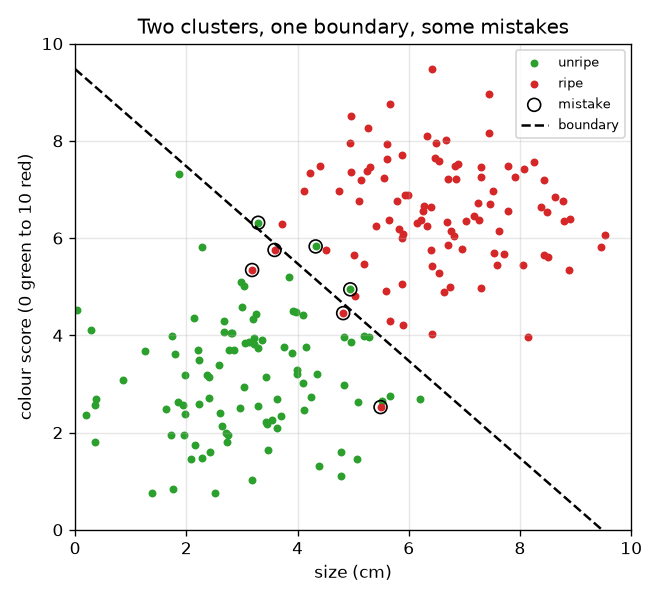
\includegraphics[width=0.85\linewidth]{figures/s01_clusters_boundary.png}\\\small Two overlapping clusters, a dashed boundary, and rings around the fruit the rule gets wrong.\end{center}

\subsection*{E. Worked example}
Twelve fruit: unripe (2, 2), (3, 4), (4, 2), (3.5, 6), (5, 3), (6, 4.5) and ripe (4.5, 7), (6, 8), (7, 6), (8, 9), (7.5, 4), (5.5, 5.5). Use the line with a = 45 degrees and c = 7. Which fruit are misclassified, and what is the accuracy?
\begin{enumerate}[nosep]
\item At 45 degrees cos = sin = 0.7071, so the rule is 0.7071 (x + y) \textgreater{} 7, that is x + y \textgreater{} 9.899.
\item Sums x + y for the unripe fruit: 4, 7, 6, 9.5, 8, 10.5. Only 10.5 (the fruit at (6, 4.5)) is above 9.899, so it is a false alarm.
\item Sums for the ripe fruit: 11.5, 14, 13, 17, 11.5, 11. All are above 9.899, so there are no misses.
\item Correct = 12 - 1 - 0 = 11, so accuracy = 11 / 12 = 0.917.
\end{enumerate}
\textbf{Answer.} One false alarm (the fruit at (6, 4.5)), no misses, accuracy 0.917.

\subsection*{F. Questions}
\begin{enumerate}[nosep]
\item \textbf{Conceptual.} Why do we count false alarms and misses separately instead of just counting 'mistakes'? Give an example where one is worse than the other.
\item \textbf{Numerical.} For the twelve fruit of the worked example, use the size-only rule 'ripe if size \textgreater{} 5' (that is a = 0 degrees, c = 5). Count the false alarms, the misses and the accuracy.
\item \textbf{Graph and simulation interpretation.} In the trade-off graph for 200 random fruit with the 45 degree boundary, what happens to the two counts as the offset c increases from 2 to 11? Where do they cross?
\item \textbf{Design and optimisation challenge.} Design: the shop says a false alarm (unripe fruit on the shelf) is worse than a miss. Should you move the boundary left or right of c = 6.7? What do you give up? How would you decide how far?
\end{enumerate}

\section{Session 2: Trees, neighbours and the confusion matrix}

\subsection*{A. Real-world problem}
A screening test for a rare condition is described as 'more than 99 percent reliable'. You test positive. How worried should you be? Surprisingly, the honest answer can be 'about one chance in six', and the reason is not the test but how rare the condition is. To see why, we need a classifier that outputs a decision, a table that counts its four outcomes, and Bayes' rule. (General education only, with made-up numbers: never personal medical advice.)

\subsection*{B. Concept and theory}
A decision tree classifies by asking a chain of yes/no questions of the form 'is feature j at most t?'. Which question? The one that makes the two resulting groups as pure as possible. For a group with a fraction p1 of class 1 and p0 = 1 - p1 of class 0, the Gini impurity is 1 - p0\textasciicircum{}2 - p1\textasciicircum{}2: 0 for a pure group and 0.5 for a 50/50 group. A split is scored by the weighted Gini of the two halves, and the best split is found by trying every feature and every midpoint between sorted values. Repeat inside each half down to a maximum depth; a depth-1 tree is a stump. k nearest neighbours keeps all the training points and votes among the k closest ones to a new point: small k gives a ragged boundary, large k a smooth one. The confusion matrix counts true positives (TP), false positives (FP), false negatives (FN) and true negatives (TN). Accuracy = (TP + TN) / total, precision = TP / (TP + FP) (of those flagged, how many were right), recall = TP / (TP + FN) (of the real positives, how many were found), and F1 = 2 TP / (2 TP + FP + FN), the harmonic mean of precision and recall. For a test with sensitivity (recall on positives) and specificity (rate of correct negatives) applied to a population with prevalence q, Bayes' rule gives the positive predictive value PPV = q sens / (q sens + (1 - q)(1 - spec)). When mistakes cost different amounts, give a score and call a case positive at or above a threshold; if the score were the true probability p, calling positive is cheaper when p is above c\_fp / (c\_fp + c\_fn).

\begin{itemize}[nosep]
\item p1: fraction of class 1 in a group (no unit)
\item G: Gini impurity of a group (no unit)
\item k: number of neighbours in the vote (count)
\item TP, FP, FN, TN: confusion matrix counts (count)
\item q: prevalence: fraction of the population that has the condition (no unit)
\item sens, spec: sensitivity and specificity of the test (no unit)
\item c\_fn, c\_fp: cost of a miss and of a false alarm (cost units)
\end{itemize}

\begin{equation*}
G = 1 - p_0^2 - p_1^2
\end{equation*}

\begin{equation*}
G_{\text{split}} = \frac{n_L\,G_L + n_R\,G_R}{n_L+n_R}
\end{equation*}

\begin{equation*}
\text{precision}=\frac{TP}{TP+FP},\quad \text{recall}=\frac{TP}{TP+FN},\quad F_1=\frac{2TP}{2TP+FP+FN}
\end{equation*}

\begin{equation*}
\text{PPV}=\frac{q\cdot\text{sens}}{q\cdot\text{sens}+(1-q)(1-\text{spec})}
\end{equation*}

\begin{equation*}
\text{call positive when } p>\frac{c_{fp}}{c_{fp}+c_{fn}}
\end{equation*}

\begin{center}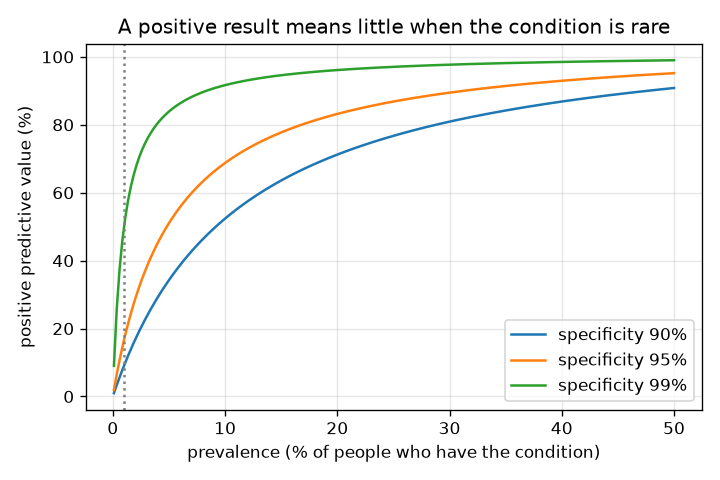
\includegraphics[width=0.85\linewidth]{figures/s02_base_rate.png}\\\small Positive predictive value against prevalence for three specificities: rare conditions give low PPV.\end{center}

\subsection*{E. Worked example}
A condition has prevalence 1 percent. The test has sensitivity 99 percent and specificity 95 percent. Of 10000 people tested, how many test positive, and what fraction of those truly have the condition?
\begin{enumerate}[nosep]
\item Have the condition: 1 percent of 10000 = 100 people. The test finds 99 percent of them: TP = 99, FN = 1.
\item Do not have it: 9900 people. The test wrongly flags 5 percent of them: FP = 0.05 x 9900 = 495, and TN = 9900 - 495 = 9405.
\item Everyone who tests positive: 99 + 495 = 594 people.
\item PPV = 99 / 594 = 0.1667, about 16.7 percent. By Bayes: 0.01 x 0.99 / (0.01 x 0.99 + 0.99 x 0.05) = 0.0099 / 0.0594 = 0.1667. The two methods agree.
\item The overall accuracy is (99 + 9405) / 10000 = 95.04 percent, yet five of every six positives are false alarms.
\end{enumerate}
\textbf{Answer.} 594 people test positive, only 99 of them truly have the condition: PPV = 16.7 percent.

\subsection*{F. Questions}
\begin{enumerate}[nosep]
\item \textbf{Conceptual.} A friend says: 'The test is 95 percent accurate, so a positive result means a 95 percent chance of having the condition.' What is wrong with this?
\item \textbf{Numerical.} A classifier produces TP = 40, FP = 10, FN = 20 and TN = 130 on 200 cases. Compute accuracy, precision, recall and F1.
\item \textbf{Graph and simulation interpretation.} On the PPV graph at prevalence 1 percent, what PPV do specificities of 90, 95 and 99 percent give (sensitivity 99 percent)? At what prevalence does a 95 percent specificity reach a PPV above 80 percent?
\item \textbf{Design and optimisation challenge.} Design: a miss costs 10 units and a false alarm costs 1 unit. You have a classifier that gives scores between 0 and 1. Why should the threshold be below 0.5, how low would the theory put it if the scores were true probabilities, and how should you choose it in practice?
\end{enumerate}

\section{Session 3: Judging a classifier honestly}

\subsection*{A. Real-world problem}
A model that scores 100 percent on its own training data can fail on new cases; a model can be accurate overall while flagging one group of people far more often than another; and a model can look brilliant only because of a bookkeeping slip. How do we judge a classifier honestly? The tools are held-out data, the ROC curve, cross-validation, group-wise error rates, and a habit of asking how a number could be fooling us. (All data are synthetic; nothing here says anything about real people.)

\subsection*{B. Concept and theory}
Most classifiers output a score and call a case positive at or above a threshold. Lower the threshold and the true-positive rate TPR = TP / (TP + FN) rises, but so does the false-positive rate FPR = FP / (FP + TN). The ROC curve plots TPR against FPR for every threshold; the area under it (AUC) equals the probability that a randomly chosen positive case scores higher than a randomly chosen negative case (ties count one half). A random forest averages many trees, each grown on a bootstrap sample (n cases drawn with replacement) and combined by majority vote; individual trees are unstable but their vote is steadier. A deeper tree can memorise noise: its training accuracy rises to 100 percent while accuracy on new data falls. K-fold cross-validation shuffles the cases into k folds and, for each fold, trains on the rest and tests on that fold, so every case is tested once. A score is calibrated if, among cases scored near 0.7, about 70 percent are positive. For fairness, compare error rates by group: if group B's scores are all shifted up by s but the ranking inside each group is the same, then with one threshold t the false-positive rates are 1 - Phi(t) and 1 - Phi(t - s), different even though AUC is equal. Two failure cases: leakage (using test data when scaling or choosing features inflates accuracy) and class imbalance (accuracy hides a useless classifier when positives are rare).

\begin{itemize}[nosep]
\item TPR: true-positive rate (recall) (no unit)
\item FPR: false-positive rate (no unit)
\item AUC: area under the ROC curve (no unit)
\item t: decision threshold on the score (score units)
\item d: separation between class centres, in score spreads (no unit)
\item s: upward shift of group B's scores (score units)
\item Phi: the standard normal cumulative distribution function (no unit)
\item k: number of cross-validation folds (count)
\end{itemize}

\begin{equation*}
\text{TPR}=\frac{TP}{TP+FN},\qquad \text{FPR}=\frac{FP}{FP+TN}
\end{equation*}

\begin{equation*}
\text{AUC}=\int_0^1 \text{TPR}\,d(\text{FPR})=P\big(\text{score}_{+}>\text{score}_{-}\big)
\end{equation*}

\begin{equation*}
\text{FPR}_A=1-\Phi(t),\qquad \text{FPR}_B=1-\Phi(t-s),\qquad \text{TPR}_g=1-\Phi(t-s_g-d)
\end{equation*}

\begin{equation*}
\text{AUC}=\Phi\!\left(\frac{d}{\sqrt{2}}\right)
\end{equation*}

\begin{center}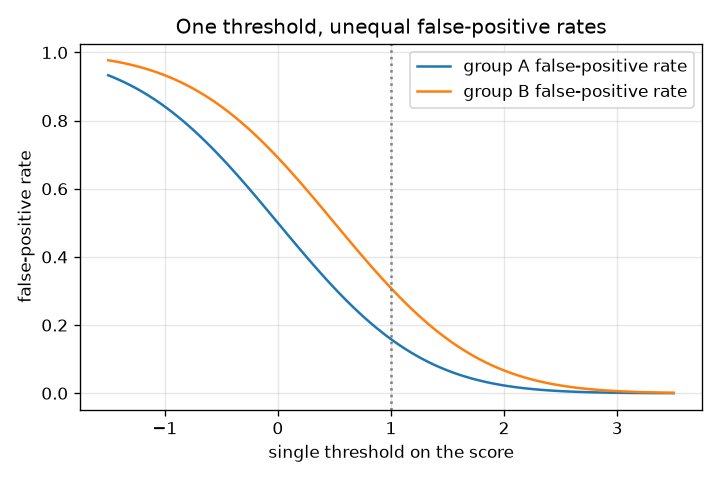
\includegraphics[width=0.85\linewidth]{figures/s03_fairness.png}\\\small One threshold, two groups: the false-positive rate curves are parallel but apart.\end{center}

\subsection*{E. Worked example}
Four cases have scores 0.1, 0.4, 0.35, 0.8 and true labels 0, 0, 1, 1. Build the ROC curve and compute the AUC by area and as a probability.
\begin{enumerate}[nosep]
\item Sort by score, highest first: 0.8 (positive), 0.4 (negative), 0.35 (positive), 0.1 (negative). There are 2 positives and 2 negatives.
\item Lower the threshold past each score and update (FPR, TPR): start (0, 0); after 0.8 -\textgreater{} (0, 0.5); after 0.4 -\textgreater{} (0.5, 0.5); after 0.35 -\textgreater{} (0.5, 1); after 0.1 -\textgreater{} (1, 1).
\item Area under the curve by trapezoids: 0 + 0.5 x 0.5 + 0 + 0.5 x 1 = 0.25 + 0.5 = 0.75.
\item Pairs (positive, negative): 0.35 \textgreater{} 0.1 yes, 0.35 \textgreater{} 0.4 no, 0.8 \textgreater{} 0.1 yes, 0.8 \textgreater{} 0.4 yes: 3 of 4 pairs, probability 0.75. The two methods agree.
\end{enumerate}
\textbf{Answer.} AUC = 0.75, both from the area under the ROC curve and as the probability that a random positive outranks a random negative.

\subsection*{F. Questions}
\begin{enumerate}[nosep]
\item \textbf{Conceptual.} Why can training accuracy reach 100 percent while test accuracy falls as a tree gets deeper? Why does a forest of trees help?
\item \textbf{Numerical.} Group B's scores are shifted up by 0.5 relative to group A, negatives are centred at 0 and the threshold is 1.0. Compute each group's false-positive rate with Phi(1) = 0.8413 and Phi(0.5) = 0.6915.
\item \textbf{Graph and simulation interpretation.} In the overfitting figure, which depth would you choose and why? What does the gap between the two curves tell you?
\item \textbf{Design and optimisation challenge.} Design: a screening problem has 5 percent positives; a miss costs 20 and a false alarm costs 1. You may choose a depth-3 tree, a depth-8 tree or a 25-tree forest and a threshold. Which would you pick and how do you justify it?
\end{enumerate}

\section{Session 4: Tune the forest by cross-validation}

\subsection*{A. Real-world problem}
In Session 3 the forest of depth 12 scored 0.716 on new cases, and the depth curve showed that a shallow tree does better. So choose the depth that scores best, no? Not on the test set: if the setting that scores best on the test set is the one you keep, the test set has helped build the model, and its score is no longer an honest forecast of future cases. Students ask how to choose the tree depth without peeking at the test set. Today we choose the depth with k-fold cross-validation on the training data only, add random feature subsets at each split, and measure two things: what the choice buys (accuracy) and what it cannot promise (the size of the error bar of a 500-case test set). All data are synthetic, and nothing here says anything about real people.

\subsection*{B. Concept and theory}
A \textbf{parameter} is learned from the data (a threshold in a tree); a \textbf{hyperparameter} is a setting chosen before learning (the depth). Hyperparameters need a third kind of data. The training set fits the model; the test set judges the final model once; and the choice of hyperparameter needs its own judge that is neither of those. Cross-validation provides it from the training data: cut the training cases into k folds, and for each depth train on k - 1 folds and score on the fold held out, rotating. The k scores of a depth give a mean and a standard error SE = s / sqrt(k), where s is their standard deviation. The \textbf{best rule} takes the depth with the highest mean (the shallower on a tie). The \textbf{one-standard-error rule} takes the shallowest depth whose mean is within one SE of the best, because scores that close cannot be told apart and simpler is safer. A real random forest also draws a random subset of the features at each split; here with two features one feature is drawn per split. Every measured accuracy has a sampling error: for p measured on n cases the standard error is sqrt(p (1 - p) / n), which is 0.019 for 500 cases. Finally the best of several noisy scores is biased upwards (a maximum is bigger than a typical value), so the winning score is optimistic. The remedy is to report the test score of the final model, measured once on cases that played no part in the choice, with its error bar.

\begin{itemize}[nosep]
\item k: number of folds (no unit)
\item a\_d,i: accuracy of depth d on held-out fold i (no unit)
\item mean, SE: mean fold score and its standard error (no unit)
\item p, n: accuracy and number of test cases (no unit and count)
\item max\_features: features examined at each split (count)
\end{itemize}

\begin{equation*}
\bar a_d=\frac1k\sum_{i=1}^{k}a_{d,i},\qquad \mathrm{SE}_d=\frac{s_d}{\sqrt k},\qquad d^\ast_{\text{one-SE}}=\min\{d:\ \bar a_d\ge \max_{d'}\bar a_{d'}-\mathrm{SE}_{\text{best}}\}
\end{equation*}

\begin{equation*}
\mathrm{SE}(\text{accuracy})=\sqrt{\frac{p\,(1-p)}{n_{\text{test}}}}
\end{equation*}

\begin{center}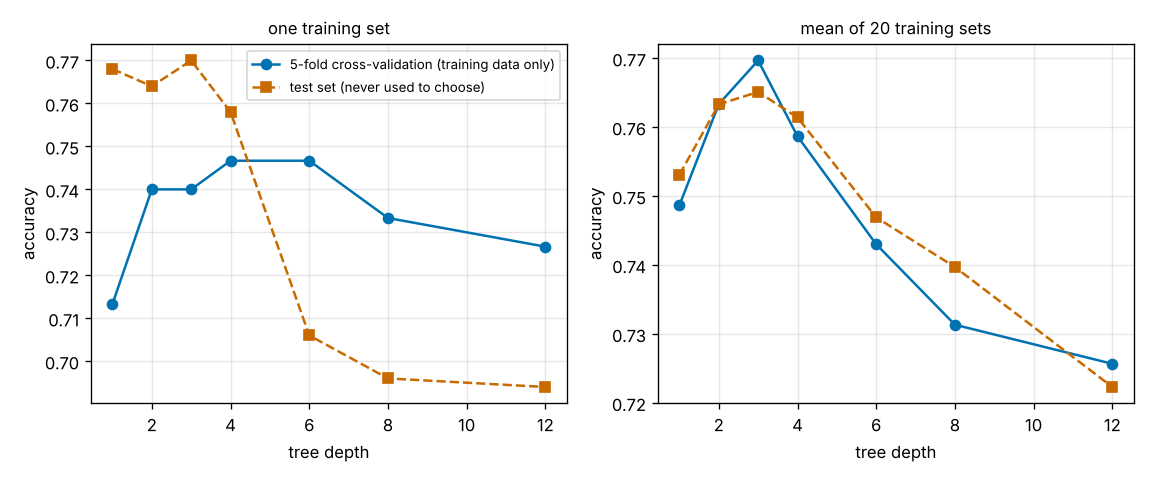
\includegraphics[width=0.95\linewidth]{figures/s04_cv_vs_test.png}\\\small Cross-validation (blue) against the test set (orange): one training set and the mean of 20.\end{center}

\begin{center}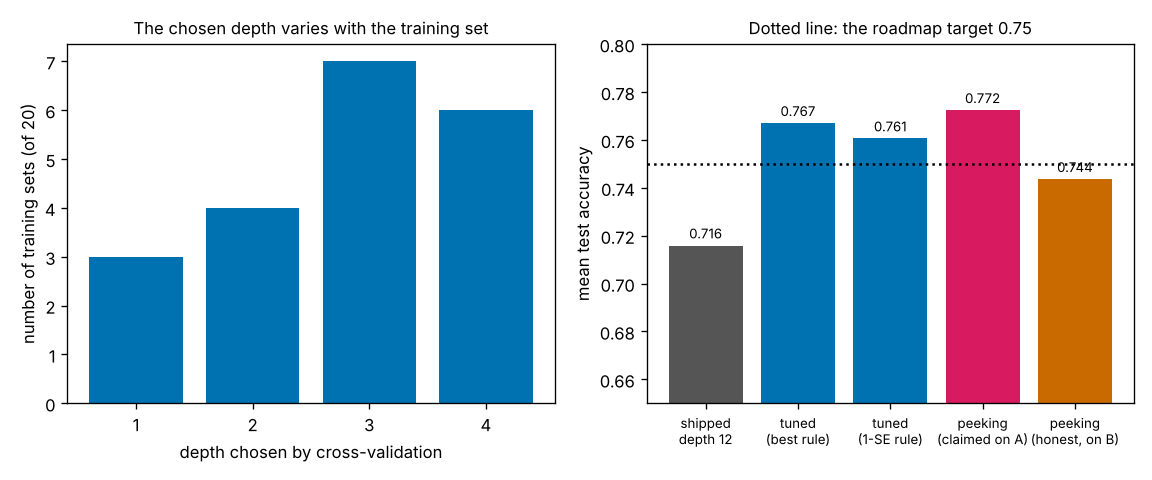
\includegraphics[width=0.95\linewidth]{figures/s04_chosen_and_accuracy.png}\\\small The 20 chosen depths and the mean test accuracy of five choices.\end{center}

\begin{center}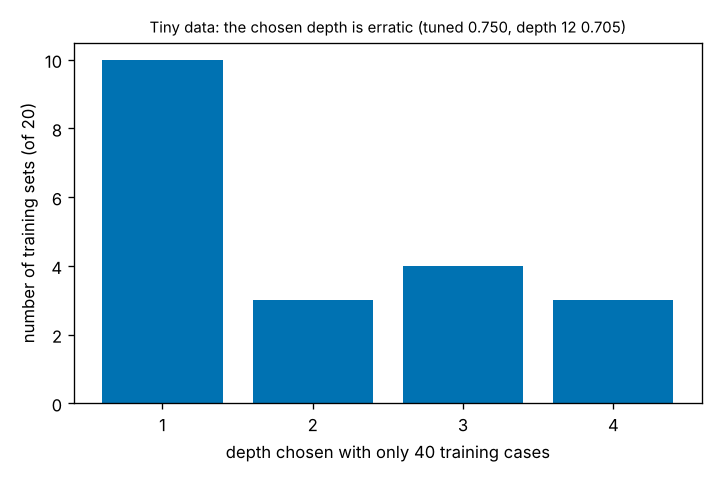
\includegraphics[width=0.6\linewidth]{figures/s04_tiny_data.png}\\\small With 40 training cases the chosen depth is erratic.\end{center}

\subsection*{E. Worked example}
Four depths are cross-validated with 5 folds and give the fold scores: depth 1: 0.70, 0.74, 0.72, 0.70, 0.74; depth 2: 0.80, 0.78, 0.78, 0.78, 0.78; depth 3: 0.82, 0.76, 0.80, 0.78, 0.79; depth 4: 0.77, 0.75, 0.74, 0.76, 0.73. Find the mean of each depth, the standard error of the best, and the depth chosen by the best rule and by the one-SE rule.
\begin{enumerate}[nosep]
\item The means are 0.720 (depth 1), 0.784 (depth 2), 0.790 (depth 3) and 0.750 (depth 4).
\item The best mean is 0.790 at depth 3; the best rule chooses depth 3.
\item The standard deviation of the depth-3 scores: the deviations from 0.79 are 0.03, -0.03, 0.01, -0.01, 0, so s = sqrt((0.0009 + 0.0009 + 0.0001 + 0.0001) / 4) = 0.0224.
\item SE = s / sqrt(5) = 0.0224 / 2.236 = 0.0100.
\item The one-SE threshold is 0.790 - 0.010 = 0.780. Depth 1 (0.720) fails; depth 2 (0.784) passes, so the one-SE rule chooses the shallowest passing depth, 2.
\end{enumerate}
\textbf{Answer.} Means 0.720, 0.784, 0.790, 0.750; SE of the best 0.010; the best rule chooses depth 3 and the one-SE rule depth 2.

\subsection*{F. Questions}
\begin{enumerate}[nosep]
\item \textbf{Conceptual.} Why must the test set not be used to choose the tree depth, and what role does each of the three sets (the training folds, the held-out fold, the test set) play when the depth is chosen by cross-validation?
\item \textbf{Numerical.} An accuracy of 0.767 is measured on 500 test cases. Give its standard error and a 95 percent interval (about plus or minus two standard errors). How many test cases would give a standard error of 0.005?
\item \textbf{Graph and simulation interpretation.} In the left panel of Figure 1 (training set 1) the cross-validation score is highest at depths 4 and 6, but test set A prefers depth 3 and the one-SE rule would take depth 2. Is cross-validation wrong here? What do the error bars say?
\item \textbf{Design and optimisation challenge.} Design: you have only 40 labelled cases and must choose the tree depth and make an honest statement about the accuracy. What do you do, and what do you tell the client?
\end{enumerate}

\section{Session 5: A threshold for each group}

\subsection*{A. Real-world problem}
In Session 3 one threshold on the score gave group A a false-positive rate of 0.159 and group B a rate of 0.309, twice as many false alarms, because B's measuring instrument reads 0.5 too high. Session 3 showed the gap and stopped. Students ask the natural question: so set a separate threshold for each group, and is that the end of it? Today we build the tool that does it and then look at what it costs. In the Session 3 setting the repair is free and removes the gap completely. It stops being free when the groups differ in how common the condition is, or in how good the instrument is, and then no choice of thresholds can satisfy every fairness definition at once. We also measure how many cases it takes to set the thresholds from data, which is more than most people expect. All data are synthetic, and nothing here says anything about real people.

\subsection*{B. Concept and theory}
A group is described by three numbers: the share of positive cases (prevalence, pi), the quality of the instrument (d, the distance between the scores of positives and negatives, in units of their spread) and the shift s, how much the instrument reads too high. With a threshold t the rates follow from the normal curve Phi: FPR = 1 - Phi(t - s) and TPR = 1 - Phi(t - s - d). The share of flagged people who really are positive, PPV, is pi x TPR divided by the flagged share. To set a wanted false-positive rate f, invert the curve: t = s + Phi\textasciicircum{}-1(1 - f). Applying this to each group with the same f is the repair: \textbf{one threshold per group}. In the Session 3 setting B's scores are A's plus 0.5, so B's threshold is A's plus 0.5 and every rate becomes equal.

Three other wishes compete with equal FPR: equal TPR, equal PPV, and a floor under every group's TPR (here 0.6). Bayes' rule gives the odds form PPV / (1 - PPV) = pi / (1 - pi) x TPR / FPR for every group. If two groups have equal TPR and FPR but a different pi, the PPV must differ. This is the heart of the impossibility result: \textbf{with different prevalence, equal FPR, equal TPR and equal PPV cannot all hold} (except for a perfect classifier). A weaker instrument for one group gives a second, separate problem: its ROC curve lies lower, so at equal FPR its TPR is lower, and reaching the floor means a higher common FPR, paid for by both groups.

In practice d and s are unknown, so each threshold is fitted from labelled data: the threshold with FPR f is the (1 - f) quantile of the group's negative scores. The fit is noisy, with standard error sqrt(f (1 - f) / n\_neg) for the FPR of each group, where n\_neg is the number of negative cases in the calibration set. Judge the result on cases that did not take part in the fit.

\begin{itemize}[nosep]
\item t, s: threshold and instrument shift (score units)
\item d: instrument quality (larger is better) (score units)
\item pi: share of positive cases (prevalence) (fraction)
\item FPR, TPR, PPV: false-positive rate, true-positive rate, positive predictive value (no unit)
\item f: wanted false-positive rate (no unit)
\item n\_neg: number of negative cases in a calibration set (count)
\end{itemize}

\begin{equation*}
\mathrm{FPR}_g=1-\Phi(t_g-s_g),\qquad \mathrm{TPR}_g=1-\Phi(t_g-s_g-d_g),\qquad t_g=s_g+\Phi^{-1}(1-f)
\end{equation*}

\begin{equation*}
\frac{\mathrm{PPV}_g}{1-\mathrm{PPV}_g}=\frac{\pi_g}{1-\pi_g}\cdot\frac{\mathrm{TPR}_g}{\mathrm{FPR}_g},\qquad \mathrm{SE}(\widehat{\mathrm{FPR}})=\sqrt{\frac{f\,(1-f)}{n_{\text{neg}}}}
\end{equation*}

\begin{center}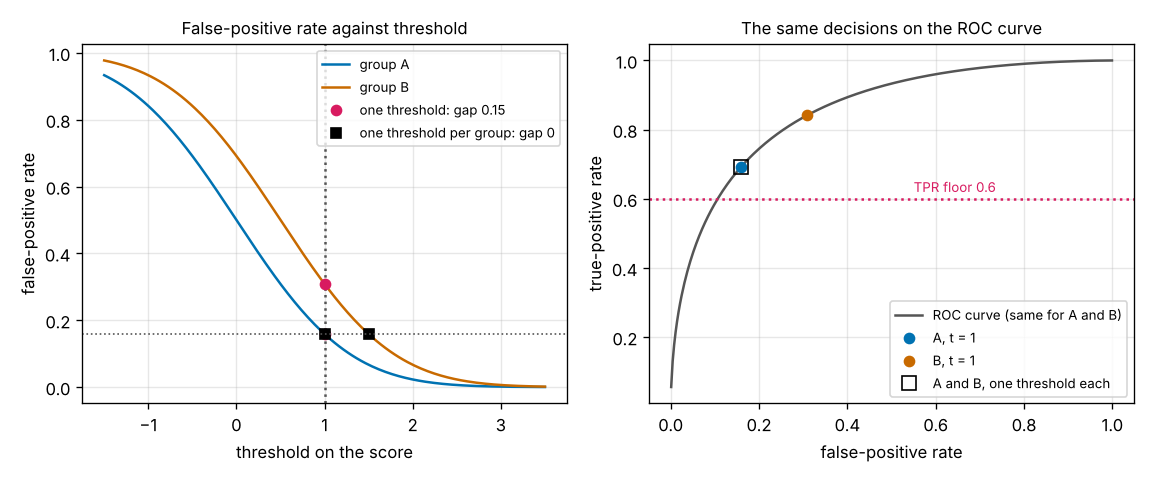
\includegraphics[width=0.95\linewidth]{figures/s05_fpr_and_roc.png}\\\small False-positive rate against threshold, and the same decisions on the ROC curve.\end{center}

\begin{center}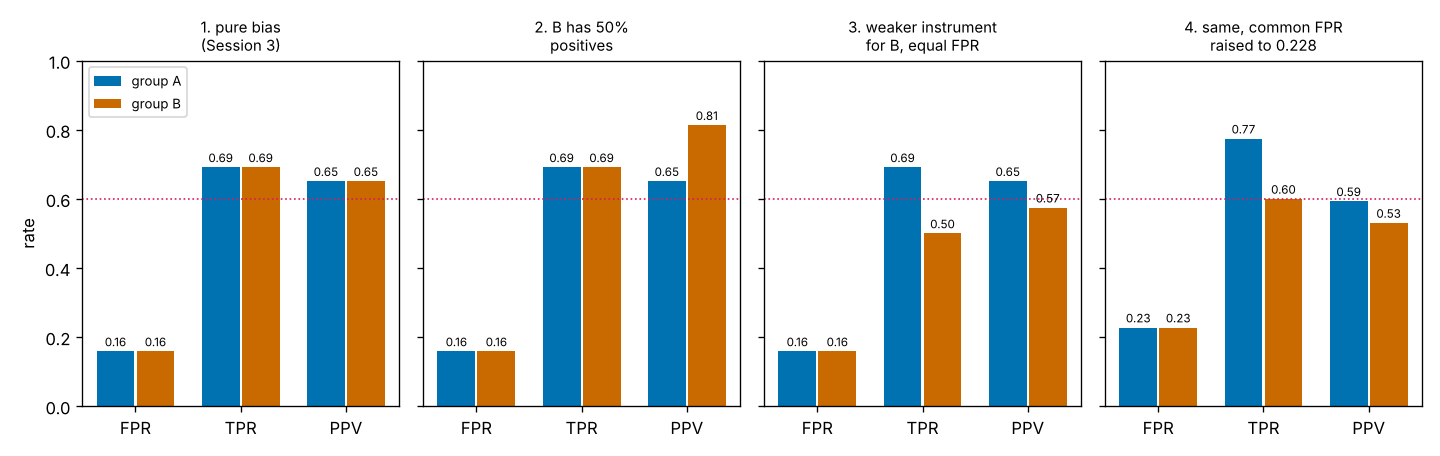
\includegraphics[width=1.0\linewidth]{figures/s05_three_situations.png}\\\small FPR, TPR and PPV of both groups in four situations.\end{center}

\begin{center}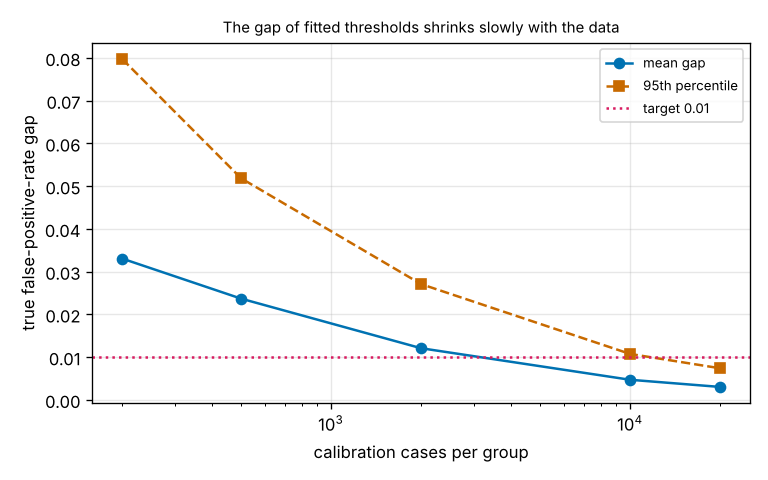
\includegraphics[width=0.6\linewidth]{figures/s05_gap_vs_size.png}\\\small The gap of fitted thresholds against the number of calibration cases.\end{center}

\subsection*{E. Worked example}
Groups A and B both have d = 1.5; B's scores are shifted up by 0.5. A single threshold t = 1 gives A a false-positive rate of 0.159. Find the threshold for B that gives it the same rate, and the true-positive rate of both groups there.
\begin{enumerate}[nosep]
\item For A at t = 1: FPR = 1 - Phi(1) = 0.1587.
\item For B we need 1 - Phi(t - 0.5) = 0.1587, so t - 0.5 = 1 and t = 1.5.
\item TPR of A at t = 1: 1 - Phi(1 - 1.5) = 1 - Phi(-0.5) = 0.6915.
\item TPR of B at t = 1.5: 1 - Phi(1.5 - 0.5 - 1.5) = 1 - Phi(-0.5) = 0.6915.
\item Both are above the floor 0.6, and the gap in the false-positive rates is 0.
\end{enumerate}
\textbf{Answer.} B's threshold is 1.5; both groups have FPR 0.159 and TPR 0.691.

\subsection*{F. Questions}
\begin{enumerate}[nosep]
\item \textbf{Conceptual.} Two groups have different shares of positive cases. Why can a classifier not give them equal false-positive rates, equal true-positive rates and equal PPV all at once, and which of the three should a clinic give up?
\item \textbf{Numerical.} Group C has prevalence 0.2, group D prevalence 0.4. Both have d = 1.5 and no shift, and both are judged at the threshold 1.0. Find the FPR, TPR and PPV of each. What TPR would D need, at the same FPR, to have the PPV of C?
\item \textbf{Graph and simulation interpretation.} In the third panel of Figure 2 the two groups have the same false-positive rate and B's true-positive rate is 0.50 against 0.69 for A. In the fourth panel the common false-positive rate is raised to 0.228. Who gains, who pays, and why can no choice of thresholds remove the difference?
\item \textbf{Design and optimisation challenge.} Design: a clinic has only 300 labelled cases from group B (prevalence 0.3) and 20000 from group A. It wants B's false-positive rate to match A's within 0.01. What do you build, and what do you promise the clinic?
\end{enumerate}

\section{Real-world mini-project}
\textbf{Choose a model and a threshold for a synthetic screening problem.} A clinic-style screening problem, entirely synthetic: 5 percent of cases are positive, a miss costs 20 units and a false alarm costs 1 unit. Use \texttt{make\_screening}, \texttt{grow\_tree}, \texttt{fit\_forest}, \texttt{pick\_threshold} and \texttt{cost\_and\_confusion} from Session 3. For each of three models (a depth-3 tree, a depth-8 tree and a 25-tree forest of depth 6), choose the threshold that minimises the cost on a validation set, then report the confusion matrix and the cost on a separate test set. General education only: this is not a medical tool.

\textbf{Report the tuned forest honestly.} Use the Session 3 experiment (20 training sets of 150 cases, test set A of 500 cases, 15 percent label noise) with the lesson's \texttt{tuning\_table}, \texttt{shipped\_accuracy}, \texttt{honest\_report} and \texttt{small\_data\_study}. The roadmap target is a mean test accuracy of at least 0.75 for the tuned forest (the shipped depth-12 forest gives 0.716). \textbf{Deliverable:} A script that picks the depth of each of the 20 training sets by 5-fold cross-validation with both rules, prints the chosen depths and the mean test accuracy next to the shipped forest, counts on how many training sets tuning wins and gives the mean gain with its standard error, repeats the comparison on a fresh test set B, measures the optimism of peeking and of the best cross-validation score, states the standard error of a 500-case accuracy, and repeats the whole thing with 40 training cases. It saves the graph of the cross-validation and test curves. \textbf{Success looks like:} The best rule gives 0.767 and the one-SE rule 0.761, both above the target 0.75; tuning wins on 19 of 20 sets with a mean gain of 0.051 (standard error 0.007); the chosen depths are all between 1 and 4. On the fresh set B the tuned forest scores 0.741 against 0.696 for the shipped one, so the gain holds although every number is lower. Peeking claims 0.772 but scores 0.744 on set B; the best cross-validation score averages 0.780. Your report says that 0.767 has a standard error of 0.019, larger than its margin of 0.017 over the target, and that the gain over the shipped forest is the safer claim. With 40 training cases the chosen depth is erratic but tuned (0.750) still beats the deep forest (0.705).

\textbf{A tool that picks one threshold per group.} Use the Session 3 settings (group A: no shift; group B: shift 0.5; d = 1.5; prevalence 0.3; 20000 cases per group) with the lesson's \texttt{threshold\_tool}, \texttt{three\_situations} and \texttt{gap\_study}. The roadmap target is a false-positive-rate gap of at most 0.01 while both true-positive rates stay at least 0.6 (the single threshold of Session 3 gives a gap of 0.15). \textbf{Deliverable:} A script that fits one threshold per group from a calibration set, prints both groups' FPR, TPR, PPV and errors per 1000 people on the test data for the single threshold and for the per-group thresholds, repeats the analysis for a different prevalence and for a weaker instrument (with and without the TPR floor), states the cost of each repair, and measures how the gap of fitted thresholds depends on the number of calibration cases. It saves the graph of the false-positive rate against the threshold. \textbf{Success looks like:} With the exact thresholds 1.0 and 1.5 the gap is 0 and both TPR are 0.691. Fitted from 20000 calibration cases per group the thresholds are 1.012 and 1.514, and on the Session 3 test data the gap falls from 0.152 to 0.005 with TPR 0.684 and 0.689. The errors of B fall from 264 to 204 per 1000 people. With 50 percent positives in B, PPV is 0.651 against 0.813 at equal FPR and TPR; equal PPV would need B's TPR to be 0.296. With a weaker instrument B's TPR is 0.50; the floor needs a common FPR of 0.228, which costs A 69 more false alarms per 1000 negative cases. The gap of fitted thresholds is at most 0.01 in 22 of 100 repeats with 200 cases per group, 41 with 2000, 91 with 10000 and 98 with 20000. Your report says that the target is met on this test set but that it is a statement about 20000 cases per group, and that a small group cannot promise it.

\section{The path ahead}
\begin{enumerate}[nosep]
\item \textbf{Session 6: Beat the screening cost.} A screening classifier chosen and tuned only with validation data.
\item \textbf{Session 7: How sure is the AUC?} A 95 percent bootstrap interval for the AUC and a coverage experiment.
\item \textbf{Session 8: Three classes and a 3 by 3 confusion matrix.} A classifier for three fruit types with a 3 by 3 matrix and macro-F1.
\end{enumerate}

\section{Answers and hints}

\subsection*{Session 1}
\begin{enumerate}[nosep]
\item \textbf{Conceptual.} Hint: Think about what each mistake costs the packing line. Solution: Both are wrong decisions, but they cost different things. Sending an unripe fruit to the shop (false alarm) loses a customer's trust; keeping a ripe fruit back (miss) wastes a good fruit. For a smoke alarm a miss (fire, no alarm) is far worse than a false alarm. The total number of mistakes hides this, so we report both.
\item \textbf{Numerical.} Hint: List the sizes of the unripe fruit and the ripe fruit and mark which are above 5. Solution: Unripe sizes: 2, 3, 4, 3.5, 5, 6; only 6 is above 5, so 1 false alarm (size exactly 5 is not above 5). Ripe sizes: 4.5, 6, 7, 8, 7.5, 5.5; only 4.5 is not above 5, so 1 miss. Correct = 12 - 2 = 10, accuracy = 10 / 12 = 0.833. Sanity check: using colour as well (the 45 degree line) did better, with only 1 mistake.
\item \textbf{Graph and simulation interpretation.} Hint: A larger c moves the line towards the ripe cluster. Solution: False alarms fall steadily (96 at c = 2, with 0 misses) because fewer fruit are called ripe, and misses rise from 0. The curves cross near c = 6.6, where the two counts are about equal. At c = 6.7 the rule makes 3 false alarms and 4 misses out of 200.
\item \textbf{Design and optimisation challenge.} Hint: Use the trade-off curves: which way does each count move? Solution: Move it right (larger c): fewer false alarms, at the price of more misses, which here means more ripe fruit kept back. To decide how far, give each mistake a cost (for example a false alarm costs 3 and a miss costs 1), compute 3 x FA + 1 x miss along the c axis and take the lowest point. Assumption: the sample is typical of the real line; with only 200 fruit the exact best c is uncertain.
\end{enumerate}

\subsection*{Session 2}
\begin{enumerate}[nosep]
\item \textbf{Conceptual.} Hint: Compare accuracy, specificity and positive predictive value. Solution: Accuracy, sensitivity and specificity describe how the test behaves on people whose true state is known. A positive result asks the reverse question: given the test result, what is the true state? That is the PPV, and it depends on prevalence as well. With 1 percent prevalence the PPV is 16.7 percent even though the overall accuracy is 95.04 percent.
\item \textbf{Numerical.} Hint: Total = 200. Use the four formulas in Section B. Solution: Accuracy = (40 + 130) / 200 = 0.85. Precision = 40 / 50 = 0.8. Recall = 40 / 60 = 0.667. F1 = 2 x 40 / (2 x 40 + 10 + 20) = 80 / 110 = 0.727. Sanity check: F1 lies between precision and recall.
\item \textbf{Graph and simulation interpretation.} Hint: Read the three curves at the x value 1; use the PPV formula to check. Solution: At 1 percent prevalence the PPV is 9.1 percent for specificity 90 percent, 16.7 percent for 95 percent and 50 percent for 99 percent. At 20 percent prevalence a specificity of 95 percent gives a PPV of 83 percent, so the curve passes 80 percent a little below a prevalence of 20 percent. The lesson: improving specificity helps most when the condition is rare.
\item \textbf{Design and optimisation challenge.} Hint: Compare the expected cost of saying positive with that of saying negative; then think about which data you may use to choose. Solution: For a case with true probability p, saying positive costs (1 - p) x 1 and saying negative costs p x 10; positive is cheaper when p \textgreater{} 1 / 11 = 0.0909. Real scores are not perfect probabilities, so search the thresholds on a separate validation set. In the code, a threshold of 4/15 = 0.267 for a k = 15 neighbour classifier gave a test cost of 55, against 90 at the default 0.5. Trade-off: a low threshold buys fewer misses with more false alarms. Assumption: the costs are right and the validation set resembles future cases.
\end{enumerate}

\subsection*{Session 3}
\begin{enumerate}[nosep]
\item \textbf{Conceptual.} Hint: Think about what a leaf holding a single noisy case has learned. Solution: A deep tree keeps splitting until every leaf is pure, so it memorises the training labels, including the noise from flipped labels; that memorised noise does not repeat in new data. A single tree is also unstable: a different training set gives a very different tree. A forest averages many trees grown on bootstrap samples, so the wobble of individual trees partly cancels, and predictions change less from one training set to the next.
\item \textbf{Numerical.} Hint: FPR\_A = 1 - Phi(t) and FPR\_B = 1 - Phi(t - s). Solution: FPR\_A = 1 - Phi(1.0) = 1 - 0.8413 = 0.1587. FPR\_B = 1 - Phi(1.0 - 0.5) = 1 - Phi(0.5) = 1 - 0.6915 = 0.3085. Group B's false-positive rate is about twice group A's. Sanity check: shifting B's scores up pushes more of its negatives over the threshold.
\item \textbf{Graph and simulation interpretation.} Hint: Never choose by training accuracy; read the test curve. Solution: Choose depth 2, where test accuracy peaks (0.7385). Beyond it the training accuracy keeps rising (100 percent by depth 15) while test accuracy falls to 0.6065 at depth 20. The widening gap between the curves is the overfitting. In practice you would pick the depth by cross-validation on the training data, not by looking at the test set.
\item \textbf{Design and optimisation challenge.} Hint: Choose the threshold on a validation set for each model, then compare the models on a separate test set. Solution: For each model pick the cheapest threshold on the validation set, then measure the cost on the test set. On the shipped data the test costs are 1360 (depth 3), 1685 (depth 8) and 1230 (forest), against 2300 for flagging nobody. Pick the forest: the deeper single tree overfits and costs more. Its confusion matrix (TP, FP, FN, TN) is (76, 450, 39, 2435): it accepts many false alarms because they are 20 times cheaper than misses. Assumptions: the costs are right and future data look like the test set.
\end{enumerate}

\subsection*{Session 4}
\begin{enumerate}[nosep]
\item \textbf{Conceptual.} Hint: What does a score on the test set mean if the test set has already decided which model you are looking at? Solution: A test score is only an honest forecast if the test cases played no part in building the model. Choosing the depth that scores best on the test set uses the test cases to build the model: among several depths, the winner is partly the one that was lucky on those 500 cases, so its score on them is too high (0.772 claimed against 0.744 on a fresh set in the lesson). Cross-validation moves the choice into the training data. The training folds fit each forest, the held-out fold judges it, and rotating the roles gives k scores per depth. The test set is not touched until one depth has been chosen; it is used once, for the final report.
\item \textbf{Numerical.} Hint: SE = sqrt(p (1 - p) / n). Solve the same formula for n. Solution: SE = sqrt(0.767 x 0.233 / 500) = sqrt(3.57e-4) = 0.0189, so the 95 percent interval is about 0.767 plus or minus 0.038, that is 0.729 to 0.805. For SE = 0.005: n = p (1 - p) / SE\textasciicircum{}2 = 0.1787 / 0.000025 = 7149, about 7100 test cases. This is why the lesson's 500-case test set can show that tuning beats the shipped forest (a paired comparison on the same cases) but cannot show that the tuned forest reaches 0.75: its margin of 0.017 is smaller than one standard error.
\item \textbf{Graph and simulation interpretation.} Hint: How long are the error bars compared with the differences between the depths from 2 to 12? Solution: No. The cross-validation scores for depths 2 to 12 lie within about 0.02 of each other and the one-standard-error bars (about 0.03 long) overlap all of them, so the data cannot tell these depths apart. The argmax simply takes the top of a flat curve (4, the shallower of the tied 4 and 6), and the test curve, which has its own noise, peaks at another point of the same plateau. Choosing 4 instead of 3 costs 0.012 on test set A, which is within the noise. What cross-validation does reliably is to rule out depth 1 and the deep forests (8, 12). The one-SE rule says this openly by choosing the shallowest depth on the plateau.
\item \textbf{Design and optimisation challenge.} Hint: Use the 40-case study of Figure 3: how erratic is the chosen depth, and what is the risk of the deep forest? Solution: Do not trust the argmax of a 5-fold score with 8 cases per fold: over 20 such data sets the chosen depth took four different values from 1 to 4. Still, tuning matters more than the exact depth: shallow forests reached 0.750 on a 2000-case test set, while the depth-12 forest got 0.705, so any depth from 1 to 4 chosen by the one-SE rule (shallowest on the plateau) is safe, and a depth chosen by the test set would be worse than useless. Report the accuracy with an error bar: an accuracy estimated from 40 cases has a standard error of about sqrt(0.75 x 0.25 / 40) = 0.07, so say 'about 0.75, give or take 0.14 (two standard errors)', and tell the client that more labelled data is the real remedy. Assumption: the same synthetic problem with 15 percent label noise.
\end{enumerate}

\subsection*{Session 5}
\begin{enumerate}[nosep]
\item \textbf{Conceptual.} Hint: Write the PPV of a group in terms of prevalence, TPR and FPR (the odds form of Section B). What happens to the right-hand side when only the prevalence changes? Solution: Bayes' rule gives PPV / (1 - PPV) = prev / (1 - prev) x TPR / FPR for every group. If two groups have equal TPR and equal FPR but different prevalence, the factor prev / (1 - prev) differs, so their PPV must differ: in the lesson 0.651 against 0.813 for prevalences 0.3 and 0.5. Forcing equal PPV at equal FPR changes a TPR instead, and the lesson shows the price: B's TPR would have to fall to 0.296. The only escapes are equal prevalence or a perfect classifier (FPR = 0 and TPR = 1), neither of which is on offer. There is no neutral answer to which to give up: it depends on which error hurts more, a missed positive (TPR), a false alarm (FPR) or a flag that means less in one group (PPV). That is a decision for the people who bear the consequences, not for the script, and the honest report shows all three numbers for both groups.
\item \textbf{Numerical.} Hint: FPR = 1 - Phi(1) and TPR = 1 - Phi(-0.5) are the same for both groups. Then PPV = prev x TPR / (prev x TPR + (1 - prev) x FPR). Solution: FPR = 1 - Phi(1) = 0.1587 and TPR = 1 - Phi(-0.5) = 0.6915 for both. Group C: flagged = 0.2 x 0.6915 + 0.8 x 0.1587 = 0.1383 + 0.1269 = 0.2652, so PPV = 0.1383 / 0.2652 = 0.521. Group D: flagged = 0.4 x 0.6915 + 0.6 x 0.1587 = 0.2766 + 0.0952 = 0.3718, so PPV = 0.2766 / 0.3718 = 0.744. The same instrument and the same threshold flag a group of 40 percent positives with a precision of 0.74 and a group of 20 percent with 0.52. For equal PPV at FPR 0.1587 the odds must match: D needs TPR = [0.521 / 0.479] x [0.6 / 0.4] x 0.1587 = 1.0898 x 1.5 x 0.1587 = 0.259, far below the 0.6 floor.
\item \textbf{Graph and simulation interpretation.} Hint: Find the two operating points on the two ROC curves (in the app, the second graph with the second preset). Solution: B gains: moving up its ROC curve from FPR 0.159 to 0.228 lifts its TPR from 0.50 to 0.60, exactly the floor. Both groups pay: with equal FPR both groups get the same 0.228, so A also receives 69 more false alarms per 1000 negative cases, although A's own TPR rises (0.69 to 0.77), and its PPV falls from 0.65 to 0.59. B's PPV falls from 0.58 to 0.53. The difference cannot be removed by thresholds because B's ROC curve lies below A's (AUC 0.76 against 0.86): at every FPR B's TPR is lower, so equal FPR and equal TPR cannot both hold. Only a better instrument for B (a larger d) changes that. The alternative of lowering A's TPR to match B (levelling down) makes the numbers equal and the service worse for everyone, which is why it is a poor remedy.
\item \textbf{Design and optimisation challenge.} Hint: How many negative cases does B have, and what is the standard error of an FPR estimated from them? Use Figure 3. Solution: B has about 210 negative cases, so the FPR at any fitted threshold has a standard error of sqrt(0.159 x 0.841 / 210) = 0.025, two and a half times the tolerance. Figure 3 and the checkpoint show the same: with 200 cases per group the gap of fitted thresholds is at most 0.01 in only 22 of 100 repeats (mean gap 0.033), and about 10000 cases per group are needed to reach 91 of 100. So build the tool as in the lesson (fit each group's threshold as a quantile of its negative scores on a calibration set, judge it on separate cases) but do not promise 0.01. Promise an interval: 'B's false-positive rate will match A's to within about plus or minus 0.05 (two standard errors)', and recommend collecting more labelled B cases, or fitting a model with fewer parameters (a normal curve for the negatives) if the assumption can be defended. Also tell the clinic that using group membership in a decision is a policy and legal question, not only a technical one. Assumption: the synthetic setting of the lesson.
\end{enumerate}

\section{How to join}
Read \texttt{CONTRIBUTING.md} in the repository, then pick an issue labelled \texttt{good first issue}. Repository: \url{https://github.com/KrunalPanchal1995/pan-iit-oss/tree/main/openclassifier}

\end{document}
